%-------------------- Document-wide settings --------------------%
\documentclass[aspectratio=1610,12pt,dvipsnames]{beamer}

\usepackage[font=small,skip=2pt]{caption}
\captionsetup[figure]{labelformat=empty}

\usetheme{Warsaw}

\setbeamertemplate{navigation symbols}{}
\setbeamertemplate{footline}
{
  \leavevmode%
  \hbox{%
  \begin{beamercolorbox}[wd=.4\paperwidth,ht=2.25ex,dp=1ex,center]{author in head/foot}%
    \usebeamerfont{author in head/foot}\insertshortauthor
  \end{beamercolorbox}%
  \begin{beamercolorbox}[wd=.6\paperwidth,ht=2.25ex,dp=1ex,center]{title in head/foot}%
    \usebeamerfont{title in head/foot}\insertshorttitle\hspace*{3em}
    \insertframenumber{} / \inserttotalframenumber\hspace*{1ex}
  \end{beamercolorbox}}%
  \vskip0pt%
}

\usepackage{listings,graphicx,verbatimbox,hyperref}
\usepackage{hyperref}
%\usepackage{bibentry}
% \usepackage[customcolors,shade]{hf-tikz}
% \usepackage{tikz}
\usepackage{amsmath}
\usepackage{xcolor}

\newcommand*{\colorboxed}{}
\def\colorboxed#1#{%
  \colorboxedAux{#1}%
}
\newcommand*{\colorboxedAux}[3]{%
  % #1: optional argument for color model
  % #2: color specification
  % #3: formula
  \begingroup
  \colorlet{cb@saved}{.}%
  \color#1{#2}%
  \boxed{%
    \color{cb@saved}%
    #3%
  }%
  \endgroup
}

\usepackage[style=nature]{biblatex}
\DeclareCiteCommand{\footcite}[\mkbibfootnote]
  {\usebibmacro{prenote}}
  {\printnames[family-given]{labelname}%
   \hspace{1mm} \printfield{journaltitle}%
   \hspace{1mm} \printfield{year}}
  {\addsemicolon\space}
  {\usebibmacro{postnote}}


\newcommand{\N}{\mathbb{N}}
\newcommand{\Z}{\mathbb{Z}}
\newcommand{\Q}{\mathbb{Q}}
\newcommand{\R}{\mathbb{R}}
\newcommand{\C}{\mathbb{C}}
\newcommand{\norm}[1]{\left\lVert#1\right\rVert}
\newcommand{\ceil}[1]{\lceil#1\rceil}
\newcommand{\ov}{\overline}
\newcommand{\cleq}{\preccurlyeq}
\newcommand{\cgeq}{\succcurlyeq}
\newcommand{\bdy}{\textbf{\text{Bdy}}}
\newcommand{\trace}{\text{trace}}
\newcommand{\dom}{\textbf{dom}}
\newcommand{\expec}{\mathbb{E}}
\newcommand{\bigO}{\mathcal{O}}
\newcommand{\tr}{\text{tr}}
\newcommand{\<}{\langle}
\renewcommand{\>}{\rangle}
\newcommand*\oldmacro{}%
\let\oldmacro\insertshorttitle%
\DeclareMathOperator*{\argmax}{arg\,max}
\DeclareMathOperator*{\argmin}{arg\,min}


\date{\today}

\addbibresource{NOGA-UA-gas/bib/gas.bib}

\begin{document}
%------------------------------------------------------------------%

%-------------------- NOGA UA Gas Modeling ------------------------%
\title[Control of Line Pack in Natural Gas System of Israel]{Control of Line Pack in Natural Gas System of Israel:
Balancing Limited Resources under Uncertainty}
\author[Hyett, Pagnier, Alisse, Saban, Goldshtein, Chertkov]{Criston Hyett, Laurent Pagnier, Jean Alisse, Lilah Saban, Igal Goldshtein, Misha Chertkov}

\institute{The University of Arizona \& NOGA Israel}

\graphicspath{{./NOGA-UA-gas/figs/}}
% -------------------------------------------------------------------------------%
\begin{frame}
  \maketitle
\end{frame}
% -------------------------------------------------------------------------------%


% -------------------------------------------------------------------------------%
\begin{frame}{Project Goals}
  \begin{itemize}
  \item Operations-aware modeling and simulation of a reduced model of Israel's natural gas network.
    \begin{itemize}
    \item Flux control at inlet nodes
    \item Realistic initial conditions
    \item Assessing relevant challenges
      \begin{itemize}
      \item Robustness in the case of uncertain PV generation
      \item Robustness in the case of an insult to the system
      \end{itemize}
    \end{itemize}

  \item Model \& open-source tool development
    \begin{itemize}
    \item Solver suite specifically suited to the needs of natural gas networks
    \item Advanced automatic controls
    \item Monte-Carlo/Uncertainty Quantification
    \end{itemize}
  \end{itemize}
\end{frame}
% -------------------------------------------------------------------------------%

% -------------------------------------------------------------------------------%
\begin{frame}{Results: Scenario 5}
  \begin{figure}
    \centering
    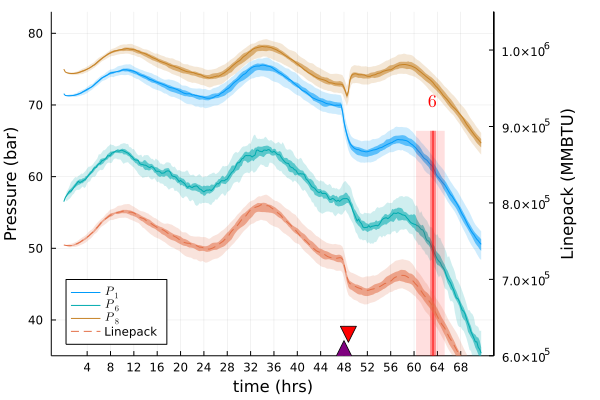
\includegraphics[width=0.65\textwidth]{ScenarioResults/scen5.png}
    \caption{Linepack and pressures for insult at hour 48, implementing a max-flow control on the remaining supply at node 8. $\tau = 14.17 \pm 4.07 \text{ hrs}$}
  \end{figure}
\end{frame}
% -------------------------------------------------------------------------------%

%-------------------------------------------------------------------------------%
\begin{frame}{Next Steps}
  \begin{itemize}
  \item Better UQ: Stochastic Finite Volumes(?)
  \item Higher order method and efficient implementation to allow for parallelization and acceleration.
  \item Advanced automatic controls
    \begin{itemize}
    \item This would mimick some actual protocol, and allow you to make statements such as, "with 95\% confidence, using protocol A, the natural gas system is robust to an insult of type B"
    \end{itemize}
  \item Simulation and optimization of the joint power and gas grids, under uncertainty.
  \end{itemize}
\end{frame}
%-------------------------------------------------------------------------------%



\end{document}